\documentclass[11pt,border=5pt]{standalone}
\usepackage{fontspec}
\setmainfont{cmunrm.otf}[BoldFont=cmunbx.otf,ItalicFont=cmunti.otf,BoldItalicFont=cmunbi.otf]
\usepackage{amsmath}
\usepackage{unicode-math}
\setmathfont{NewCMMath-Regular.otf}
\usepackage{tikz}
\usetikzlibrary{arrows.meta,patterns,angles,quotes}
\begin{document}
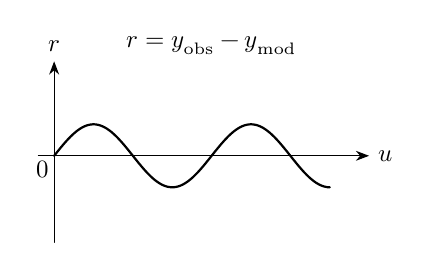
\begin{tikzpicture}[>=Stealth,font=\small,line cap=round,line join=round]
\draw[->,thin] (-0.2,0) -- (4,0) node[right] {$u$};
\draw[->,thin] (0,-1.1) -- (0,1.2) node[above] {$r$};
\node at (-0.14,-0.18) {$0$};
\draw[thick] plot coordinates {(0.00000,0.00000) (0.02917,0.03660) (0.05833,0.07289) (0.08750,0.10858) (0.11667,0.14335) (0.14583,0.17692) (0.17500,0.20900) (0.20417,0.23933) (0.23333,0.26765) (0.26250,0.29373) (0.29167,0.31734) (0.32083,0.33829) (0.35000,0.35640) (0.37917,0.37152) (0.40833,0.38353) (0.43750,0.39231) (0.46667,0.39781) (0.49583,0.39997) (0.52500,0.39877) (0.55417,0.39422) (0.58333,0.38637) (0.61250,0.37528) (0.64167,0.36103) (0.67083,0.34376) (0.70000,0.32361) (0.72917,0.30074) (0.75833,0.27534) (0.78750,0.24764) (0.81667,0.21786) (0.84583,0.18625) (0.87500,0.15307) (0.90417,0.11862) (0.93333,0.08316) (0.96250,0.04701) (0.99167,0.01047) (1.02083,-0.02616) (1.05000,-0.06257) (1.07917,-0.09846) (1.10833,-0.13352) (1.13750,-0.16746) (1.16667,-0.20000) (1.19583,-0.23086) (1.22500,-0.25978) (1.25417,-0.28652) (1.28333,-0.31086) (1.31250,-0.33259) (1.34167,-0.35153) (1.37083,-0.36752) (1.40000,-0.38042) (1.42917,-0.39014) (1.45833,-0.39658) (1.48750,-0.39969) (1.51667,-0.39945) (1.54583,-0.39586) (1.57500,-0.38895) (1.60417,-0.37877) (1.63333,-0.36542) (1.66250,-0.34900) (1.69167,-0.32965) (1.72083,-0.30754) (1.75000,-0.28284) (1.77917,-0.25578) (1.80833,-0.22656) (1.83750,-0.19545) (1.86667,-0.16269) (1.89583,-0.12858) (1.92500,-0.09338) (1.95417,-0.05740) (1.98333,-0.02093) (2.01250,0.01570) (2.04167,0.05221) (2.07083,0.08828) (2.10000,0.12361) (2.12917,0.15790) (2.15833,0.19086) (2.18750,0.22223) (2.21667,0.25173) (2.24583,0.27912) (2.27500,0.30416) (2.30417,0.32666) (2.33333,0.34641) (2.36250,0.36326) (2.39167,0.37706) (2.42083,0.38769) (2.45000,0.39508) (2.47917,0.39914) (2.50833,0.39986) (2.53750,0.39723) (2.56667,0.39126) (2.59583,0.38201) (2.62500,0.36955) (2.65417,0.35400) (2.68333,0.33547) (2.71250,0.31413) (2.74167,0.29015) (2.77083,0.26374) (2.80000,0.23511) (2.82917,0.20452) (2.85833,0.17220) (2.88750,0.13845) (2.91667,0.10353) (2.94583,0.06774) (2.97500,0.03138) (3.00417,-0.00524) (3.03333,-0.04181) (3.06250,-0.07804) (3.09167,-0.11361) (3.12083,-0.14822) (3.15000,-0.18160) (3.17917,-0.21345) (3.20833,-0.24350) (3.23750,-0.27152) (3.26667,-0.29726) (3.29583,-0.32050) (3.32500,-0.34106) (3.35417,-0.35875) (3.38333,-0.37343) (3.41250,-0.38498) (3.44167,-0.39330) (3.47083,-0.39832) (3.50000,-0.40000)};
\node at (2,1.4) {$r=y_{\rm obs}-y_{\rm mod}$};

\end{tikzpicture}
\end{document}
